% answers.tex —— 2002 年·北京卷·理科 · 参考答案与详细解析片段
% 由 tools/generate_projects.py 依来源总账自 2002/2002_数学真题_北京理_试题.md + 2002/2002_数学真题_北京理_解析正文.md + 2002/2002_数学真题_北京理_答案要点.md 生成，勿手改（改源 MD 后重跑）


\begin{gktip}
固定来源 PDF 没有答案页。以下为本项目根据固定题面独立推导，不是官方答案或官方解析。Q16 原圆方程无实点，故答案保留 U/PENDING；Q18、Q19 的原文疑点不在解析中静默修订。
\end{gktip}

\gkpart{一、选择题}

\begin{answer}
\gksolhead{1}{}

\textbf{题目}：

满足条件 \(M\cup\{1\}=\{1,2,3\}\) 的集合 \(M\) 的个数是\mbox{（　　）}。

（A）1　　（B）2　　（C）3　　（D）4

\Needspace{4\baselineskip}
\textbf{解析}

由 \(M\cup\{1\}=\{1,2,3\}\)，必须有 \(2,3\in M\)，且 \(M\subseteq\{1,2,3\}\)。元素 1 可取可不取，因此只有 \(M=\{2,3\}\) 或 \(M=\{1,2,3\}\) 两种，选 B。

\gkanswer{答案：B（2）。}

\end{answer}
\begin{answer}
\gksolhead{2}{}

\textbf{题目}：

在平面直角坐标系中，已知两点 \(A(\cos80^\circ,\sin80^\circ)\)，\(B(\cos20^\circ,\sin20^\circ)\)，则 \(|AB|\) 的值是\mbox{（　　）}。

（A）\(\dfrac12\)　　（B）\(\dfrac{\sqrt2}{2}\)　　（C）\(\dfrac{\sqrt3}{2}\)　　（D）1

\Needspace{4\baselineskip}
\textbf{解析}

\Needspace{5\baselineskip}
两点都在单位圆上，对应圆心角为 \(80^\circ-20^\circ=60^\circ\)，所以弦长
\nopagebreak[4]
\[
|AB|=2\sin30^\circ=1.
\]
选 D。

\gkanswer{答案：D（1）。}

\end{answer}
\begin{answer}
\gksolhead{3}{}

\textbf{题目}：

下列四个函数中，以 \(\pi\) 为最小正周期，且在区间 \(\left(\dfrac\pi2,\pi\right)\) 上为减函数的是\mbox{（　　）}。

（A）\(y=\cos^2x\)　　（B）\(y=2|\sin x|\)　　（C）\(y=\left(\dfrac13\right)^{\cos x}\)　　（D）\(y=-\cot x\)

\Needspace{4\baselineskip}
\textbf{解析}

\(\cos^2x\) 在 \((\pi/2,\pi)\) 上递增；\(2|\sin x|\) 在该区间递减且最小正周期为 \(\pi\)；\((1/3)^{\cos x}\) 随 \(x\) 增大而递增；\(-\cot x\) 的导数为 \(\csc^2x>0\)，也递增。因此只有 B 符合。

\gkanswer{答案：B。}

\end{answer}
\begin{answer}
\gksolhead{4}{}

\textbf{题目}：

64 个直径都为 \(\dfrac a4\) 的球，记它们的体积之和为 \(V_{\text{甲}}\)，表面积之和为 \(S_{\text{甲}}\)；一个直径为 \(a\) 的球，记其体积为 \(V_{\text{乙}}\)，表面积为 \(S_{\text{乙}}\)，则\mbox{（　　）}。

（A）\(V_{\text{甲}}>V_{\text{乙}},\ S_{\text{甲}}>S_{\text{乙}}\)　　（B）\(V_{\text{甲}}<V_{\text{乙}},\ S_{\text{甲}}<S_{\text{乙}}\)

（C）\(V_{\text{甲}}=V_{\text{乙}},\ S_{\text{甲}}>S_{\text{乙}}\)　　（D）\(V_{\text{甲}}=V_{\text{乙}},\ S_{\text{甲}}=S_{\text{乙}}\)

\Needspace{4\baselineskip}
\textbf{解析}

小球半径是大球半径的 \(1/4\)。64 个小球的总体积与大球体积之比为 \(64(1/4)^3=1\)，总表面积与大球表面积之比为 \(64(1/4)^2=4\)。故体积相等而小球总表面积较大，选 C。

\gkanswer{答案：C。}

\end{answer}
\begin{answer}
\gksolhead{5}{}

\textbf{题目}：

\Needspace{5\baselineskip}
已知某曲线的参数方程是
\nopagebreak[4]
\[
\begin{cases}
x=\sec\varphi,\\
y=\tan\varphi,
\end{cases}
\quad(\varphi\text{ 为参数}),
\]
若以原点为极点，\(x\) 轴的正半轴为极轴，长度单位不便变，建立极坐标系，则该曲线的极坐标方程是\mbox{（　　）}。

（A）\(\rho=1\)　　（B）\(\rho\cos2\theta=1\)　　（C）\(\rho^2\sin2\theta=1\)　　（D）\(\rho^2\cos2\theta=1\)

\Needspace{4\baselineskip}
\textbf{解析}

\Needspace{5\baselineskip}
由参数方程及恒等式 \(\sec^2\varphi-\tan^2\varphi=1\)，有 \(x^2-y^2=1\)。代入 \(x=\rho\cos\theta,\ y=\rho\sin\theta\)，得
\nopagebreak[4]
\[
x^2-y^2=\rho^2(\cos^2\theta-\sin^2\theta)=\rho^2\cos2\theta=1.
\]
选 D。题干“长度单位不便变”按原文保留，未作题面修订。

\gkanswer{答案：D。}

\end{answer}
\begin{answer}
\gksolhead{6}{}

\textbf{题目}：

给定四条曲线：① \(x^2+y^2=\dfrac52\)，② \(\dfrac{x^2}{9}+\dfrac{y^2}{4}=1\)，③ \(x^2+\dfrac{y^2}{4}=1\)，④ \(\dfrac{x^2}{4}+y^2=1\)。其中与直线 \(x+y-\sqrt5=0\) 仅有一个交点的曲线是\mbox{（　　）}。

（A）①②③　　（B）②③④　　（C）①②④　　（D）①③④

\Needspace{4\baselineskip}
\textbf{解析}

对椭圆 \(x^2/a^2+y^2/b^2=1\)，直线 \(x+y=\sqrt5\) 的支撑值为 \(\sqrt{a^2+b^2}\)；支撑值等于 \(\sqrt5\) 时相切，大于 \(\sqrt5\) 时相交于两点。①圆的最大 \(x+y\) 为 \(\sqrt5\)；③、④的 \(a^2+b^2\) 均为 5，均相切；②的最大值为 \(\sqrt{13}>\sqrt5\)，与直线有两个交点。故恰有一个交点的是①③④，选 D。

\gkanswer{答案：D（①③④）。}

\end{answer}
\begin{answer}
\gksolhead{7}{}

\textbf{题目}：

已知 \(z_1,z_2\in\mathbb C\)，且 \(|z_1|=1\)。若 \(z_1+z_2=2\)，则 \(|z_1-z_2|\) 的最大值是\mbox{（　　）}。

（A）6　　（B）5　　（C）4　　（D）3

\Needspace{4\baselineskip}
\textbf{解析}

\Needspace{5\baselineskip}
由 \(z_2=2-z_1\)，
\nopagebreak[4]
\[
|z_1-z_2|=2|z_1-1|\leqslant2(|z_1|+1)=4.
\]
当 \(z_1=-1\) 时取等号，最大值为 4，选 C。

\gkanswer{答案：C（4）。}

\end{answer}
\begin{answer}
\gksolhead{8}{}

\textbf{题目}：

若 \(\dfrac{\cot\theta-1}{2\cot\theta+1}=1\)，则 \(\dfrac{\cos2\theta}{1+\sin2\theta}\) 的值为\mbox{（　　）}。

（A）3　　（B）\(-3\)　　（C）\(-2\)　　（D）\(-\dfrac12\)

\Needspace{4\baselineskip}
\textbf{解析}

\Needspace{5\baselineskip}
令 \(t=\cot\theta\)。由
\nopagebreak[4]
\[
\frac{t-1}{2t+1}=1
\]
\Needspace{5\baselineskip}
得 \(t=-2\)，且分母不为零。于是
\nopagebreak[4]
\[
\cos2\theta=\frac{t^2-1}{t^2+1}=\frac35,\qquad
\sin2\theta=\frac{2t}{t^2+1}=-\frac45,
\]
从而 \(\dfrac{\cos2\theta}{1+\sin2\theta}=3\)，选 A。

\gkanswer{答案：A（3）。}

\end{answer}
\begin{answer}
\gksolhead{9}{}

\textbf{题目}：

12 名学生分别到三个不同的路口进行车流量的调查，若每个路口 4 人，则不同的分配方案共有\mbox{（　　）}。

（A）\(\mathrm C_{12}^{4}\mathrm C_8^{4}\mathrm C_4^{4}\) 种　　（B）\(3\mathrm C_{12}^{4}\mathrm C_8^{4}\mathrm C_4^{4}\) 种

（C）\(\mathrm C_{12}^{4}\mathrm C_8^{4}\mathrm A_3^{3}\) 种　　（D）\(\dfrac{\mathrm C_{12}^{4}\mathrm C_8^{4}\mathrm C_4^{4}}{\mathrm A_3^{3}}\) 种

\Needspace{4\baselineskip}
\textbf{解析}

\Needspace{5\baselineskip}
三个路口互不相同。依次从12人中选4人、从余下8人中选4人，最后4人全部进入最后一个路口，方案数为
\nopagebreak[4]
\[
\binom{12}{4}\binom84\binom44.
\]
对应 A。

\gkanswer{答案：A。}

\end{answer}
\begin{answer}
\gksolhead{10}{}

\textbf{题目}：

设命题甲：“直四棱柱 \(ABCD-A_1B_1C_1D_1\) 中，平面 \(ACB_1\) 与对角面 \(BB_1D_1D\) 垂直”；命题乙：“直四棱柱 \(ABCD-A_1B_1C_1D_1\) 是正方体”，那么，甲是乙的\mbox{（　　）}。

（A）充分必要条件　　（B）充分非必要条件

（C）必要非充分条件　　（D）即非充分又非必要条件

\Needspace{4\baselineskip}
\textbf{解析}

\Needspace{5\baselineskip}
在底面内令 \(\mathbf u=\overrightarrow{AC}\)、\(\mathbf d=\overrightarrow{BD}\)，并取竖直方向为 \(\mathbf k=(0,0,h)\)。平面 \(ACB_1\) 由 \(\mathbf u\) 与 \(\overrightarrow{AB_1}\) 张成；平面 \(BB_1D_1D\) 由 \(\mathbf d\) 与 \(\mathbf k\) 张成。取两平面的法向量分别为
\nopagebreak[4]
\[
\mathbf n_1=\mathbf u\times\overrightarrow{AB_1},\qquad
\mathbf n_2=\mathbf d\times\mathbf k.
\]
\Needspace{5\baselineskip}
设底面坐标为平面 \(z=0\)，记 \(\mathbf u=(u_x,u_y,0)\)、\(\mathbf d=(d_x,d_y,0)\)，且 \(\overrightarrow{AB_1}=(v_x,v_y,h)\)，则
\nopagebreak[4]
\[
\mathbf n_1=(hu_y,-hu_x,u_xv_y-u_yv_x),\qquad
\mathbf n_2=(hd_y,-hd_x,0),
\]
因此 \(\mathbf n_1\cdot\mathbf n_2=h^2(\mathbf u\cdot\mathbf d)\)。两平面垂直当且仅当 \(AC\perp BD\)。正方形的两条对角线互相垂直，所以乙推出甲；非正方形菱形的两条对角线也互相垂直，但底面不是正方形，故甲不能推出乙。选 C。

\gkanswer{答案：C（必要非充分条件）。}

\end{answer}
\begin{answer}
\gksolhead{11}{}

\textbf{题目}：

已知 \(f(x)\) 是定义在 \((-3,3)\) 上的奇函数，当 \(0<x<3\) 时，\(f(x)\) 的图象如图所示，那么不等式 \(f(x)\cos x<0\) 的解集是\mbox{（　　）}。
\nopagebreak[4]
\begin{center}% 第 11 题源图的定性重绘：定义域为 0<x<3，零点为 x=1 与开区间端点 x=3。
% 曲线形态与端点来自固定 PDF 第 1 页；坐标比例为示意，不作为函数条件。
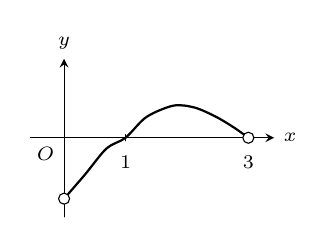
\begin{tikzpicture}[x=.78cm,y=.85cm,>=stealth,line cap=round,line join=round,
  every node/.style={font=\scriptsize}]
  \draw[->] (-.55,0)--(3.42,0) node[right] {$x$};
  \draw[->] (0,-1.18)--(0,1.18) node[above] {$y$};
  \node[below left] at (0,0) {$O$};
  \draw (.0,.045)--(.0,-.045);
  \draw (1,.045)--(1,-.045) node[below=2pt] {$1$};
  \draw (3,.045)--(3,-.045) node[below=2pt] {$3$};
  \draw[thick] plot[smooth] coordinates {
    (0,-.91) (.34,-.55) (.69,-.16) (1,0) (1.34,.31)
    (1.78,.48) (2.13,.45) (2.48,.31) (2.77,.15) (3,0)
  };
  \filldraw[fill=white] (0,-.91) circle[radius=2pt];
  \filldraw[fill=white] (3,0) circle[radius=2pt];
\end{tikzpicture}
\end{center}
\nopagebreak[4]
（A）\(\left(-3,-\dfrac\pi2\right)\cup(0,1)\cup\left(\dfrac\pi2,3\right)\)

（B）\(\left(-\dfrac\pi2,-1\right)\cup(0,1)\cup\left(\dfrac\pi2,3\right)\)

（C）\((-3,-1)\cup(0,1)\cup(1,3)\)　　（D）\(\left(-3,-\dfrac\pi2\right)\cup(0,1)\cup(1,3)\)

\Needspace{4\baselineskip}
\textbf{解析}

\Needspace{5\baselineskip}
由原图，在 \((0,1)\) 上 \(f(x)<0\)，在 \((1,3)\) 上 \(f(x)>0\)。利用奇函数性质，在 \((-3,-1)\) 上 \(f(x)<0\)，在 \((-1,0)\) 上 \(f(x)>0\)。在定义域 \((-3,3)\) 内，\(\cos x>0\) 的区间为 \((-\pi/2,\pi/2)\)，而 \(\cos x<0\) 的区间为 \((-3,-\pi/2)\cup(\pi/2,3)\)。逐段判断乘积为负，得到
\nopagebreak[4]
\[
\left(-\frac\pi2,-1\right)\cup(0,1)\cup\left(\frac\pi2,3\right).
\]
选 B。

\gkanswer{答案：B。}

\end{answer}
\gkpart{二、填空题}

\begin{answer}
\gksolhead{12}{}

\textbf{题目}：

如图所示，\(f_i(x)\ (i=1,2,3,4)\) 是定义在 \([0,1]\) 上的四个函数，其中满足性质：“对 \([0,1]\) 中任意的 \(x_1\) 和 \(x_2\)，任意 \(\lambda\in[0,1]\)，\(f[\lambda x_1+(1-\lambda)x_2]\leqslant\lambda f(x_1)+(1-\lambda)f(x_2)\) 恒成立”的只有\mbox{（　　）}。
\nopagebreak[4]
\begin{center}% 第 12 题四幅函数图的源图结构重绘；曲线高度与弯曲程度仅示意。
% 虚线 x=1 只出现在 f_2、f_3、f_4 面板，与固定 PDF 第 1 页一致。
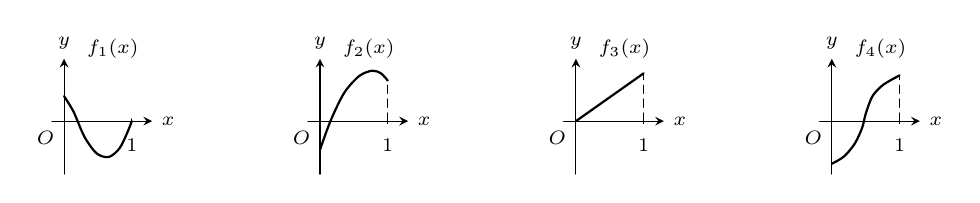
\begin{tikzpicture}[x=.86cm,y=.66cm,>=stealth,line cap=round,line join=round,
  every node/.style={font=\scriptsize}]
\foreach \shift/\name in {0/{f_1(x)},3.25/{f_2(x)},6.50/{f_3(x)},9.75/{f_4(x)}} {
  \begin{scope}[xshift=\shift cm]
    \draw[->] (-.18,0)--(1.30,0) node[right] {$x$};
    \draw[->] (0,-1.02)--(0,1.20) node[above] {$y$};
    \node[below left] at (0,0) {$O$};
    \draw (1,.045)--(1,-.045) node[below=2pt] {$1$};
    \node[above] at (.72,1.02) {$\name$};
  \end{scope}
}
% f_1：先降后升，右端在 x=1 处回到 x 轴；无辅助虚线。
\begin{scope}
  \draw[thick] plot[smooth] coordinates {
    (0,.48) (.14,.18) (.30,-.30) (.48,-.62) (.66,-.69)
    (.82,-.52) (.94,-.20) (1,0)
  };
\end{scope}
% f_2：从负值起始，凹向下上升并在 x=1 处收尾。
\begin{scope}[xshift=3.25cm]
  \draw[thick] plot[smooth] coordinates {
    (0,-.55) (.16,.02) (.36,.55) (.58,.87) (.77,.97) (.90,.92) (1,.78)
  };
  \draw[densely dashed] (1,0)--(1,.78);
\end{scope}
% f_3：从原点出发的线段，右端为 x=1。
\begin{scope}[xshift=6.50cm]
  \draw[thick] (0,0)--(1,.92);
  \draw[densely dashed] (1,0)--(1,.92);
\end{scope}
% f_4：下凸后上凸的 S 形曲线，穿过 x 轴后到达 x=1 端点。
\begin{scope}[xshift=9.75cm]
  \draw[thick] plot[smooth] coordinates {
    (0,-.82) (.18,-.68) (.34,-.43) (.45,-.12) (.50,.14)
    (.60,.48) (.76,.70) (1,.88)
  };
  \draw[densely dashed] (1,0)--(1,.88);
\end{scope}
\end{tikzpicture}
\end{center}
\nopagebreak[4]
（A）\(f_1(x),f_3(x)\)　　（B）\(f_2(x)\)　　（C）\(f_2(x),f_3(x)\)　　（D）\(f_4(x)\)

\Needspace{4\baselineskip}
\textbf{解析}

四个函数图象中，\(f_1\) 为凸形，满足凸函数的中点弦性质；\(f_3\) 是直线，也满足凸性不等式。\(f_2\) 为凹形，\(f_4\) 含有拐点，不满足在整个区间上的凸性。因此选项 A。

\gkanswer{答案：A（\(f_1(x),f_3(x)\)）。}

\end{answer}
\begin{answer}
\gksolhead{13}{}

\textbf{题目}：

\(\arcsin\left(-\dfrac25\right),\ \arccos\left(-\dfrac34\right),\ \arctan\left(-\dfrac54\right)\) 从小到大的顺序是\gkblank{}。

\Needspace{4\baselineskip}
\textbf{解析}

\Needspace{5\baselineskip}
三个数中，\(\arctan(-5/4)<0\)，而 \(\arccos(-3/4)>0\)。又
\nopagebreak[4]
\[
\tan\left(\arcsin\frac25\right)=\frac{2}{\sqrt{21}}<\frac54
\]
\Needspace{5\baselineskip}
且正切函数在 \((0,\pi/2)\) 上递增，所以 \(\arcsin(2/5)<\arctan(5/4)\)。两边取相反数，得到
\nopagebreak[4]
\[
\arctan(-5/4)<\arcsin(-2/5)<\arccos(-3/4).
\]

\gkanswer{答案：\(\arctan(-\dfrac54)<\arcsin(-\dfrac25)<\arccos(-\dfrac34)\)。}

\end{answer}
\begin{answer}
\gksolhead{14}{}

\textbf{题目}：

等差数列 \(\{a_n\}\) 中，\(a_1=2\)，公差不为零，且 \(a_1,a_3,a_{11}\) 恰好是某等比数列的前三项，那么该等比数列公比的值等于\gkblank{}。

\Needspace{4\baselineskip}
\textbf{解析}

\Needspace{5\baselineskip}
设等差数列公差为 \(d\ne0\)，则 \(a_1=2\)、\(a_3=2+2d\)、\(a_{11}=2+10d\)。它们依次为某等比数列前三项，故
\nopagebreak[4]
\[
(2+2d)^2=2(2+10d)
\quad\Longrightarrow\quad
4d(d-3)=0.
\]
由 \(d\ne0\) 得 \(d=3\)，前三项为 \(2,8,32\)，公比为 4。

\gkanswer{答案：4。}

\end{answer}
\begin{answer}
\gksolhead{15}{}

\textbf{题目}：

关于直角 \(AOB\) 在平面 \(\alpha\) 内的射影有如下判断：①可能是 \(0^\circ\) 的角；②可能是锐角；③可能是直角；④可能是直角；⑤可能是 \(180^\circ\) 的角。其中正确的序号是\gkblank{}。（注：把你认为正确判断的序号都填上。）

\begin{gktip}
原件 Q15 中③、④均印作“可能是直角”；此处按固定 PDF 原文照录，未推测或改正。
\end{gktip}

\Needspace{4\baselineskip}
\textbf{解析}

\Needspace{5\baselineskip}
设直角两边的单位方向向量为 \(\mathbf u,\mathbf v\)，其中 \(\mathbf u\cdot\mathbf v=0\)，投影平面的单位法向量为 \(\mathbf n\)。投影向量的内积为
\nopagebreak[4]
\[
\bigl(\mathbf u-(\mathbf u\cdot\mathbf n)\mathbf n\bigr)\cdot
\bigl(\mathbf v-(\mathbf v\cdot\mathbf n)\mathbf n\bigr)
=-(\mathbf u\cdot\mathbf n)(\mathbf v\cdot\mathbf n).
\]
取单位向量 \(\mathbf w\) 垂直于 \(\mathbf u,\mathbf v\)。令投影平面法向量为 \(\mathbf w\)，两边投影仍垂直；令法向量为 \((\mathbf u-\mathbf v+\mathbf w)/\sqrt3\)，则两投影内积为正且不共线，可得锐角。法向量取 \((\mathbf u-\mathbf v)/\sqrt2\) 时两投影同向，得到 \(0^\circ\)；取 \((\mathbf u+\mathbf v)/\sqrt2\) 时两投影反向，得到 \(180^\circ\)。因此五个判断均可能成立。③、④原件重复印作“可能是直角”，故两个序号都填。

\gkanswer{答案：①②③④⑤。}

\end{answer}
\begin{answer}
\gksolhead{16}{}

\textbf{题目}：

已知 \(P\) 是直线 \(3x+4y+8=0\) 上的动点，\(PA,PB\) 是圆 \(x^2+y^2-2x-2y+8=0\) 的两条切线，\(A,B\) 是切点，\(C\) 是圆心，那么四边形 \(PACB\) 面积的最小值为\gkblank{}。

\Needspace{4\baselineskip}
\textbf{解析}

\Needspace{5\baselineskip}
原方程满足
\nopagebreak[4]
\[
x^2+y^2-2x-2y+8=0
\quad\Longleftrightarrow\quad
(x-1)^2+(y-1)^2=-6.
\]
实数平方和不可能为负，故该方程没有实点，不存在题目所称的圆、切点及四边形面积。原式按固定题面保留，答案记为 U/PENDING；取得可追溯的同版勘误或更强来源前，不改系数、不猜答案。

\gkanswer{答案：U/PENDING。}

\end{answer}
\gkpart{三、解答题}

\begin{answer}
\gksolhead{17}{}

\textbf{题目}：

解不等式 \(\left|\sqrt{2x-1}-x\right|<2\)。

\Needspace{4\baselineskip}
\textbf{解析}

\Needspace{5\baselineskip}
定义域为 \(x\geqslant1/2\)。令 \(t=\sqrt{2x-1}\geqslant0\)，则 \(x=(t^2+1)/2\)，并且
\nopagebreak[4]
\[
\sqrt{2x-1}-x=t-\frac{t^2+1}{2}=-\frac{(t-1)^2}{2}.
\]
故原不等式等价于 \((t-1)^2<4\)。结合 \(t\geqslant0\)，得 \(t<3\)，即 \(x<5\)。所以解集为 \([1/2,5)\)。

\gkanswer{答案：\([\dfrac12,5)\)。}

\end{answer}
\begin{answer}
\gksolhead{18}{}

\textbf{题目}：

如图，在多面体 \(ABCD-A_1B_1C_1D_1\) 中，上、下底面平行且均为矩形，相对的侧面与同一底面所成的二面角大小相等，侧棱延长后相交与 \(E,F\) 两点。上、下底面矩形的长、宽分别为 \(c,d\) 与 \(a,b\)，且 \(a>c,b>d\)，两底面间的距离为 \(h\)。

（1） 求侧面 \(ABB_1A_1\) 与底面 \(ABCD\) 所成二面角的大小；

（2） 证明：\(EF\parallel ABCD\)；

\Needspace{5\baselineskip}
（3） 在估侧该多面体的体积时，经常运用近似公式 \(V_{\text{估}}=S_{\text{中截面}}\cdot h\) 来计算，已知它的体积公式是
\nopagebreak[4]
\[
V=\frac{h}{6}\left(S_{\text{上底面}}+4S_{\text{中截面}}+S_{\text{下底面}}\right),
\]
试判断 \(V_{\text{估}}\) 与 \(V\) 的大小关系，并加以证明。

注：与两个底面平行，且到两个底面距离相等的截面称为该多面体的中截面。
\nopagebreak[4]
\begin{center}% 第 18 题多面体源图的拓扑重绘：上下底面为矩形，侧棱延长形成 E、F。
% 所有长度比例仅为示意；尺寸标签 a,b,c,d 保留，图中不增添 h。
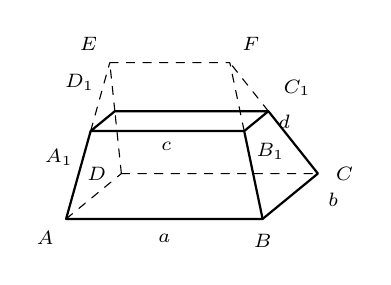
\begin{tikzpicture}[x=.78cm,y=.72cm,line cap=round,line join=round,
  every node/.style={font=\scriptsize}]
  \coordinate (A)  at (0,0);
  \coordinate (B)  at (3.2,0);
  \coordinate (C)  at (4.1,.8);
  \coordinate (D)  at (.9,.8);
  \coordinate (A1) at (.4,1.55);
  \coordinate (B1) at (2.9,1.55);
  \coordinate (C1) at (3.294,1.9);
  \coordinate (D1) at (.794,1.9);
  \coordinate (E)  at (.711,2.756);
  \coordinate (F)  at (2.666,2.756);

  % 可见棱
  \draw[thick] (A)--(B)--(C)--(C1)--(B1)--(A1)--(D1)--(C1);
  \draw[thick] (A)--(A1) (B)--(B1);
  % 隐藏棱
  \draw[dashed] (A)--(D) (D)--(C) (D)--(D1);
  % 侧棱延长线及交点 E、F；与源图一样用虚线表示。
  \draw[dashed] (A1)--(E) (D1)--(E) (B1)--(F) (C1)--(F) (E)--(F);

  % 源图尺寸标签仅标在线段附近，不画尺寸箭头。
  \node at (1.6,-.34) {$a$};
  \node at (4.35,.33) {$b$};
  \node at (1.63,1.28) {$c$};
  \node at (3.55,1.72) {$d$};

  \node[below left=1pt] at (A) {$A$};
  \node[below=2pt] at (B) {$B$};
  \node[right=3pt] at (C) {$C$};
  \node[left=2pt] at (D) {$D$};
  \node[below left=3pt] at (A1) {$A_1$};
  \node[below right=1pt] at (B1) {$B_1$};
  \node[above right=2pt] at (C1) {$C_1$};
  \node[above left=4pt] at (D1) {$D_1$};
  \node[above left=1pt] at (E) {$E$};
  \node[above right=1pt] at (F) {$F$};
\end{tikzpicture}
\end{center}
\nopagebreak[4]
\Needspace{4\baselineskip}
\textbf{解析}

\gksubpart{(1) 二面角}

\Needspace{5\baselineskip}
设下底面在 \(z=0\) 平面内，取
\nopagebreak[4]
\[
A=(0,0,0),\quad B=(a,0,0),\quad C=(a,b,0),\quad D=(0,b,0),
\]
\Needspace{5\baselineskip}
并写上底面为
\nopagebreak[4]
\[
A_1=(s,t,h),\quad B_1=(s+c,t,h),\quad
C_1=(s+c,t+d,h),\quad D_1=(s,t+d,h).
\]
\Needspace{5\baselineskip}
侧面 \(ABB_1A_1\) 与底面的二面角由垂直于 \(AB\) 的截面确定，其水平位移为 \(|t|\)；相对侧面 \(DCC_1D_1\) 的对应位移为 \(|t+d-b|\)。两二面角大小相等且 \(b>d\)，所以 \(|t|=|t+d-b|\)，从而 \(t=(b-d)/2\)。于是
\nopagebreak[4]
\[
\tan\theta=\frac{h}{t}=\frac{2h}{b-d},\qquad
\theta=\arctan\frac{2h}{b-d}.
\]

\gksubpart{(2) 证明 \(EF\parallel ABCD\)}

\Needspace{5\baselineskip}
对另一对相对侧面同理，由 \(a>c\) 得 \(s=(a-c)/2\)。令 \(\lambda=\dfrac{b}{b-d}\)。直线 \(AA_1\) 上参数为 \(\lambda\) 的点是 \((\lambda s,\lambda t,\lambda h)\)；直线 \(DD_1\) 上同一参数的点为 \((\lambda s,b-\lambda t,\lambda h)\)。由于 \(\lambda t=b/2\)，这两点重合，故
\nopagebreak[4]
\[
E=(\lambda s,b/2,\lambda h).
\]
\Needspace{5\baselineskip}
同理，直线 \(BB_1\) 与 \(CC_1\) 在同一参数处相交于
\nopagebreak[4]
\[
F=(a-\lambda s,b/2,\lambda h).
\]
因此 \(E,F\) 具有相同的 \(y,z\) 坐标，直线 \(EF\) 平行于底面 \(ABCD\)。题设称其为两点，故按 \(E\ne F\) 的情形作线段论证。

\gksubpart{(3) 体积比较}

\Needspace{5\baselineskip}
中截面为矩形，边长分别为 \((a+c)/2\) 和 \((b+d)/2\)，故
\nopagebreak[4]
\[
S_{\text{中截面}}=\frac{(a+c)(b+d)}4.
\]
\Needspace{5\baselineskip}
于是
\nopagebreak[4]
\[
\begin{aligned}
V-V_{\text{估}}
&=\frac h6\left(ab+4S_{\text{中截面}}+cd\right)-hS_{\text{中截面}}\\
&=\frac h6\left(ab+cd-2S_{\text{中截面}}\right)\\
&=\frac{h(a-c)(b-d)}{12}>0,
\end{aligned}
\]
其中 \(a>c,b>d,h>0\)。所以 \(V_{\text{估}}<V\)。

\gkanswer{答案（1）：\(\theta=\arctan\dfrac{2h}{b-d}\)。}

\gkanswer{答案（2）：\(EF\parallel ABCD\)。}

\gkanswer{答案（3）：\(V_{\text{估}}<V\)。}

\end{answer}
\begin{answer}
\gksolhead{19}{}

\textbf{题目}：

\Needspace{5\baselineskip}
数列 \(\{a_n\}\) 由下列条件确定：\(x_1=a>0\)，
\nopagebreak[4]
\[
x_{n+1}=\frac12\left(x_n+\frac{a}{x_n}\right),\quad n\in\mathbb N.
\]

（1） 证明：对 \(n\geqslant2\)，总有 \(x_n\geqslant\sqrt a\)；

（2） 证明：对 \(n\geqslant2\)，总有 \(x_n\geqslant x_{n+1}\)；

（3） 若数列 \(\{a_n\}\) 的极限存在，且大于零，求 \(\lim_{n\to\infty}x_n\) 的值。

\Needspace{4\baselineskip}
\textbf{解析}

\gksubpart{(1) 下界}

\Needspace{5\baselineskip}
由 \(a>0\) 及算术—几何平均不等式，
\nopagebreak[4]
\[
x_2=\frac12\left(a+1\right)\geqslant\sqrt a.
\]
\Needspace{5\baselineskip}
若 \(x_n>0\)，则
\nopagebreak[4]
\[
x_{n+1}-\sqrt a=\frac{(x_n-\sqrt a)^2}{2x_n}\geqslant0.
\]
因此 \(x_n\geqslant\sqrt a\) 对所有 \(n\geqslant2\) 成立。

\gksubpart{(2) 单调性}

\Needspace{5\baselineskip}
当 \(n\geqslant2\) 时，
\nopagebreak[4]
\[
x_n-x_{n+1}=\frac{x_n^2-a}{2x_n}\geqslant0,
\]
其中不等式由第（1）问及 \(x_n>0\) 得出。

\gksubpart{(3) 极限}

\Needspace{5\baselineskip}
由前两问，\(x_n\) 从 \(n=2\) 起单调不增且以下界 \(\sqrt a>0\) 有界，故极限 \(L\) 存在且 \(L\geqslant\sqrt a>0\)。对递推式取极限，
\nopagebreak[4]
\[
L=\frac12\left(L+\frac aL\right),
\]
所以 \(L^2=a\)，结合 \(L>0\) 得 \(L=\sqrt a\)。题面本问的条件文字指称 \(\{a_n\}\)，而递推只定义 \(x_n\)；这里未将两种符号静默统一，结论只针对题目明确询问的递推数列 \(x_n\)。

\gkanswer{答案（1）：\(x_n\geqslant\sqrt a\quad(n\geqslant2)\)。}

\gkanswer{答案（2）：\(x_n\geqslant x_{n+1}\quad(n\geqslant2)\)。}

\gkanswer{答案（3）：\(\displaystyle\lim_{n\to\infty}x_n=\sqrt a\)。}

\end{answer}
\begin{answer}
\gksolhead{20}{}

\textbf{题目}：

\Needspace{5\baselineskip}
在研究并行计算的基本算法时，有以下简单模型问题：用计算机求 \(n\) 个不同的数 \(v_1,v_2,\ldots,v_n\) 的和
\nopagebreak[4]
\[
\sum_{i=1}^{n}v_i=v_1+v_2+\cdots+v_n,
\]
计算开始前，\(n\) 个数存贮在 \(n\) 台由网络连接的计算机中，每台机器存一个数。计算开始后，在一个单位时间内，每台机器至多到一台其他机器中读数据，并与自己原有数据相加得到新的数据，各台机器可同时完成上述工作。为了用尽可能少的单位时间，即可完成计算，方法可用下表表示（表中「1 读」「1 果」分别表示第一单位时间的被读机号与结果，其余类推；表头为排印缩写，原页为「第一单位时间·被读机号」等全称）：

\begin{center}
\begingroup\setlength{\tabcolsep}{4pt}
\begin{tabular}{cccccccc}
\toprule
机器号 & 初始 & 1 读 & 1 果 & 2 读 & 2 果 & 3 读 & 3 果 \\
\midrule
1 & \(v_1\) & 2 & \(v_1+v_2\) &  &  &  &  \\
2 & \(v_2\) & 1 & \(v_2+v_1\) &  &  &  &  \\
\bottomrule
\end{tabular}
\endgroup
\end{center}

（1） 当 \(n=4\) 时，至少需要多少个单位时间可完成计算？把你设计的方法填入下表：

\begin{center}
\begingroup\setlength{\tabcolsep}{4pt}
\begin{tabular}{cccccccc}
\toprule
机器号 & 初始 & 1 读 & 1 果 & 2 读 & 2 果 & 3 读 & 3 果 \\
\midrule
1 & \(v_1\) &  &  &  &  &  &  \\
2 & \(v_2\) &  &  &  &  &  &  \\
3 & \(v_3\) &  &  &  &  &  &  \\
4 & \(v_4\) &  &  &  &  &  &  \\
\bottomrule
\end{tabular}
\endgroup
\end{center}

（2） 当 \(n=128\) 时，要使所有机器都得到 \(\displaystyle\sum_{i=1}^{n}v_i\)，至少需要多少个单位时间可完成计算？（结论不要求证明）

\Needspace{4\baselineskip}
\textbf{解析}

\gksubpart{(1) 四台机器}

第一单位时间，机器1读2、机器2读1，机器3读4、机器4读3。第二单位时间，机器1读3、机器2读3，机器3读1、机器4读1。每轮读到的都是该轮开始时对方已有的数据；第二轮结束后四台机器都得到总和。题目表格可填为：

\begin{center}
\begingroup\setlength{\tabcolsep}{4pt}
\begin{tabular}{cccccccc}
\toprule
机器号 & 初始 & 1 读 & 1 果 & 2 读 & 2 果 & 3 读 & 3 果 \\
\midrule
1 & \(v_1\) & 2 & \(v_1+v_2\) & 3 & \(v_1+v_2+v_3+v_4\) &  &  \\
2 & \(v_2\) & 1 & \(v_2+v_1\) & 3 & \(v_2+v_1+v_3+v_4\) &  &  \\
3 & \(v_3\) & 4 & \(v_3+v_4\) & 1 & \(v_3+v_4+v_1+v_2\) &  &  \\
4 & \(v_4\) & 3 & \(v_4+v_3\) & 1 & \(v_4+v_3+v_1+v_2\) &  &  \\
\bottomrule
\end{tabular}
\endgroup
\end{center}

一轮内任一机器最多合并两个原始数据，故至少需要两轮；上表给出两轮可行方案，因此最少为两轮。

\gksubpart{(2) 一百二十八台机器}

每轮每台机器读取另一台机器的数据，已知输入数最多翻倍；经过 \(k\) 轮，一台机器最多汇集 \(2^k\) 个初始数据，所以 \(2^k\geqslant128\)，即 \(k\geqslant7\)。按机器编号 \(0,1,\ldots,127\)，第 \(j\) 轮让每台机器读取编号与自己按位异或 \(2^{j-1}\) 的机器（\(j=1,\ldots,7\)），每轮合并两份不相交数据块。七轮后所有机器都获得总和，故最少七轮。

\gkanswer{答案（1）：至少2个单位时间；一种填表方法见解析。}

\gkanswer{答案（2）：7个单位时间。}

\end{answer}
\begin{answer}
\gksolhead{21}{}

\textbf{题目}：

已知 \(O(0,0),B(1,0),C(b,c)\) 是 \(\triangle OBC\) 的三个顶点。

（1） 写出 \(\triangle OBC\) 的重心 \(G\)、外心 \(F\)、垂心 \(H\) 的坐标，并证明 \(G,F,H\) 三点共线；

（2） 当直线 \(FH\) 与 \(OB\) 平行时，求顶点 \(C\) 的轨迹。

\Needspace{4\baselineskip}
\textbf{解析}

\gksubpart{(1) 坐标与共线}

\Needspace{5\baselineskip}
三角形非退化要求 \(c\ne0\)。重心为
\nopagebreak[4]
\[
G=\left(\frac{1+b}{3},\frac c3\right).
\]
\Needspace{5\baselineskip}
设外心为 \(F=(p,q)\)。由 \(FO=FB\) 得 \(p=1/2\)；再由 \(FO=FC\) 得
\nopagebreak[4]
\[
F=\left(\frac12,\frac{b^2+c^2-b}{2c}\right).
\]
\Needspace{5\baselineskip}
高线 \(CH\perp OB\)，故 \(x_H=b\)；又 \(OH\perp BC\)，所以 \(b(b-1)+cy_H=0\)，从而
\nopagebreak[4]
\[
H=\left(b,\frac{b(1-b)}c\right).
\]
直接计算可得 \(H=3G-2F\)，故 \(G,F,H\) 共线。

\gksubpart{(2) 轨迹}

\Needspace{5\baselineskip}
当 \(FH\parallel OB\) 时，\(F,H\) 纵坐标相等，因此
\nopagebreak[4]
\[
\frac{b^2+c^2-b}{2c}=\frac{b(1-b)}c
\quad\Longleftrightarrow\quad
c^2=3b(1-b).
\]
\Needspace{5\baselineskip}
由 \(c\ne0\) 得 \(0<b<1\)。当 \((b,c)=(1/2,\pm\sqrt3/2)\) 时，\(OBC\) 为正三角形，\(F=H\)，直线 \(FH\) 不存在，须排除。因此轨迹为
\nopagebreak[4]
\[
c^2=3b(1-b),\quad 0<b<1,\quad (b,c)\ne\left(\frac12,\pm\frac{\sqrt3}{2}\right).
\]

\gkanswer{答案（1）：\(G(\frac{1+b}{3},\frac c3)\)，\(F(\frac12,\frac{b^2+c^2-b}{2c})\)，\(H(b,\frac{b(1-b)}c)\)；三点共线。}

\gkanswer{答案（2）：\(c^2=3b(1-b)\)，\(0<b<1\)，并排除 \((b,c)=(\frac12,\pm\frac{\sqrt3}{2})\)。}

\end{answer}
\begin{answer}
\gksolhead{22}{}

\textbf{题目}：

\Needspace{5\baselineskip}
已知 \(f(x)\) 是定义在 \(\mathbb R\) 上的不恒为零的函数，且对于任意的 \(a,b\in\mathbb R\) 都满足：
\nopagebreak[4]
\[
f(a\cdot b)=af(b)+bf(a).
\]

（1） 求 \(f(0),f(1)\) 的值；

（2） 判断 \(f(x)\) 的奇偶性，并证明你的结论；

（3） 若 \(f(2)=2\)，\(u_n=\dfrac{f(2^{-n})}{n}\ (n\in\mathbb N)\)，求数列 \(\{u_n\}\) 的前 \(n\) 项的和 \(S_n\)。

\Needspace{4\baselineskip}
\textbf{解析}

\gksubpart{(1) 两个函数值}

取 \(a=0,b=2\)，有 \(f(0)=2f(0)\)，所以 \(f(0)=0\)。取 \(a=b=1\)，则 \(f(1)=2f(1)\)，所以 \(f(1)=0\)。

\gksubpart{(2) 奇偶性}

\Needspace{5\baselineskip}
取 \(a=b=-1\)，由 \(f(1)=-2f(-1)\) 得 \(f(-1)=0\)。再取 \(a=-1,b=x\)，则
\nopagebreak[4]
\[
f(-x)=-f(x)+xf(-1)=-f(x),
\]
故 \(f\) 为奇函数。

\gksubpart{(3) 前 \(n\) 项和}

\Needspace{5\baselineskip}
由 \(f(2)=2\) 开始归纳：若 \(f(2^k)=k2^k\)，则
\nopagebreak[4]
\[
f(2^{k+1})=2^k f(2)+2f(2^k)=2^{k+1}+k2^{k+1}=(k+1)2^{k+1}.
\]
\Needspace{5\baselineskip}
所以 \(f(2^k)=k2^k\)（\(k\geqslant1\)）。取 \(a=2^n,b=2^{-n}\)，则
\nopagebreak[4]
\[
0=f(1)=2^nf(2^{-n})+2^{-n}f(2^n)
=2^nf(2^{-n})+n,
\]
\Needspace{5\baselineskip}
故 \(f(2^{-n})=-n2^{-n}\)，即 \(u_n=-2^{-n}\)。所以
\nopagebreak[4]
\[
S_n=-\sum_{k=1}^{n}2^{-k}=2^{-n}-1.
\]

\gkanswer{答案（1）：\(f(0)=f(1)=0\)。}

\gkanswer{答案（2）：\(f(x)\) 为奇函数。}

\gkanswer{答案（3）：\(\displaystyle S_n=2^{-n}-1\)。}

\end{answer}